\documentclass[11pt]{article}
\usepackage[margin=1in]{geometry}
\usepackage{enumitem}
\usepackage{hyperref}
\usepackage{graphicx}
\usepackage{array}
\usepackage{multicol}
\usepackage{longtable}
\usepackage{titlesec}
\usepackage{float}

\begin{document}

%==================================================
\begin{center}
    \large \textbf{Sri Sivasubramaniya Nadar College of Engineering, Chennai} \\
    (An Autonomous Institution Affiliated to Anna University) \\
    \vspace{0.3cm}
\end{center}

\begin{table}[!h]
\renewcommand{\arraystretch}{1.5}
\resizebox{\textwidth}{!}{%
\begin{tabular}{|l|cll|}
\hline
Degree \& Branch & \multicolumn{1}{c|}{B.E. Computer Science \& Engineering} & Semester & VI \\ \hline
Subject Code \& Name & \multicolumn{3}{c|}{UCS2612 -- Machine Learning Algorithms Laboratory} \\ \hline
Academic Year & 2025--2026 (Even) & Batch & 2023--2027 \\ \hline
Name & Mehanth T & Register No. & 3122235001080 \\ \hline
Due Date & \multicolumn{3}{c|}{27 February 2026} \\ \hline
\end{tabular}
}
\end{table}

\begin{center}
\textbf{Experiment 3: Regression Analysis using Linear and Regularized Models}
\end{center}

%==================================================
\section*{Objective}
To implement linear and regularized regression models for predicting a continuous target variable, evaluate their performance using multiple metrics, visualize model behavior, and analyze overfitting, underfitting, and bias--variance characteristics.

%==================================================
\section*{Dataset}
A real-world regression dataset containing numerical and categorical features related to loan applications is used.  
The target variable is the \textbf{Loan Sanction Amount (USD)}.

Dataset reference:
\begin{itemize}
    \item Kaggle: \href{https://www.kaggle.com/datasets/phileinsophos/predict-loan-amount-data}{Predict Loan Amount Data}
\end{itemize}

The dataset consists of 30,000 instances with 24 attributes, including 'Income (USD)', 'Loan Amount Request (USD)', 'Credit Score', 'Property Price', etc.
Preprocessing involved handling missing values (mean/mode imputation), one-hot encoding categorical variables, and standardizing numerical features. The data was split into training (80\%) and validation (20\%) sets.

%==================================================
\section*{Brief Theory (For Lab Understanding)}

\subsection*{Linear Regression}
Linear Regression models the relationship between input features and a continuous target variable.
It is simple, interpretable, and serves as a baseline regression model.

\subsection*{Regularized Regression Models}
Regularization techniques are used to control model complexity:
\begin{itemize}
    \item Ridge Regression reduces coefficient magnitudes
    \item Lasso Regression performs feature selection
    \item Elastic Net combines Ridge and Lasso behavior
\end{itemize}

Regularization helps improve generalization and reduce overfitting.

%==================================================
\section*{Task Description}
Students must:
\begin{itemize}
    \item Implement Linear, Ridge, Lasso, and Elastic Net regression models
    \item Tune regularization hyperparameters using Grid Search or Randomized Search
    \item Visualize regression results and errors
    \item Analyze overfitting, underfitting, and bias--variance trade-off
\end{itemize}

%==================================================
\section*{Implementation Steps}
\begin{enumerate}[label=\arabic*.]
    \item Load the dataset
    \item Perform data preprocessing:
    \begin{itemize}
        \item Handle missing values
        \item Encode categorical variables
        \item Standardize numerical features
    \end{itemize}
    \item Perform Exploratory Data Analysis (EDA)
    \item Visualize feature distributions and target distribution
    \item Split the dataset into training and testing sets
    \item Train baseline Linear Regression
    \item Train Ridge, Lasso, and Elastic Net models
    \item Perform hyperparameter tuning using 5-Fold Cross-Validation
    \item Evaluate all models using regression metrics
\end{enumerate}

%==================================================
\section*{5. Visualizations}

\subsection*{5.1 Exploratory Data Analysis}
\begin{figure}[H]
    \centering
    \includegraphics[width=0.7\textwidth]{plots/png/target_distribution.png}
    \caption{Distribution of Loan Sanction Amount}
\end{figure}

\begin{figure}[H]
    \centering
    \includegraphics[width=0.8\textwidth]{plots/png/correlation_heatmap.png}
    \caption{Correlation Heatmap}
\end{figure}

\subsection*{5.2 Model Evaluation}
\begin{figure}[H]
    \centering
    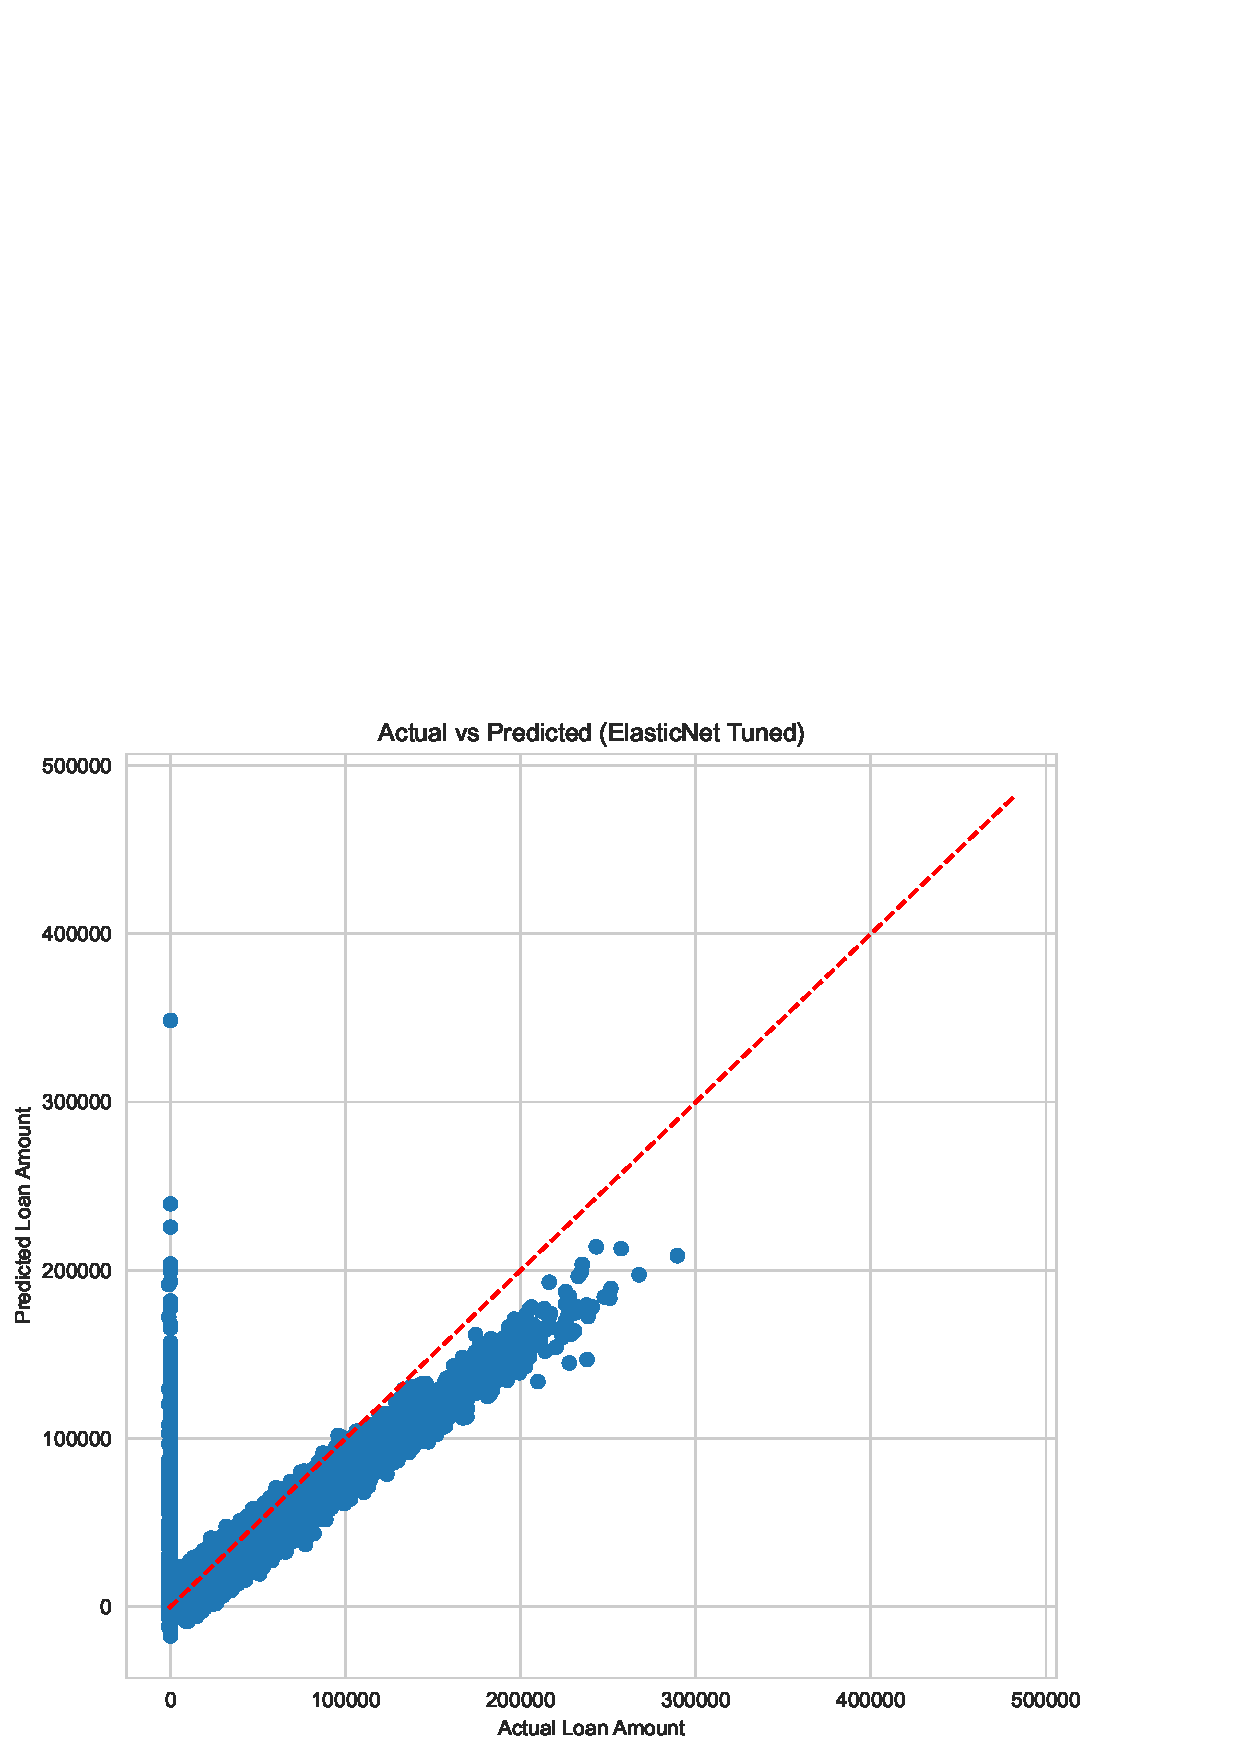
\includegraphics[width=0.6\textwidth]{plots/png/predicted_vs_actual.png}
    \caption{Predicted vs Actual Values (Best Model)}
\end{figure}

\begin{figure}[H]
    \centering
    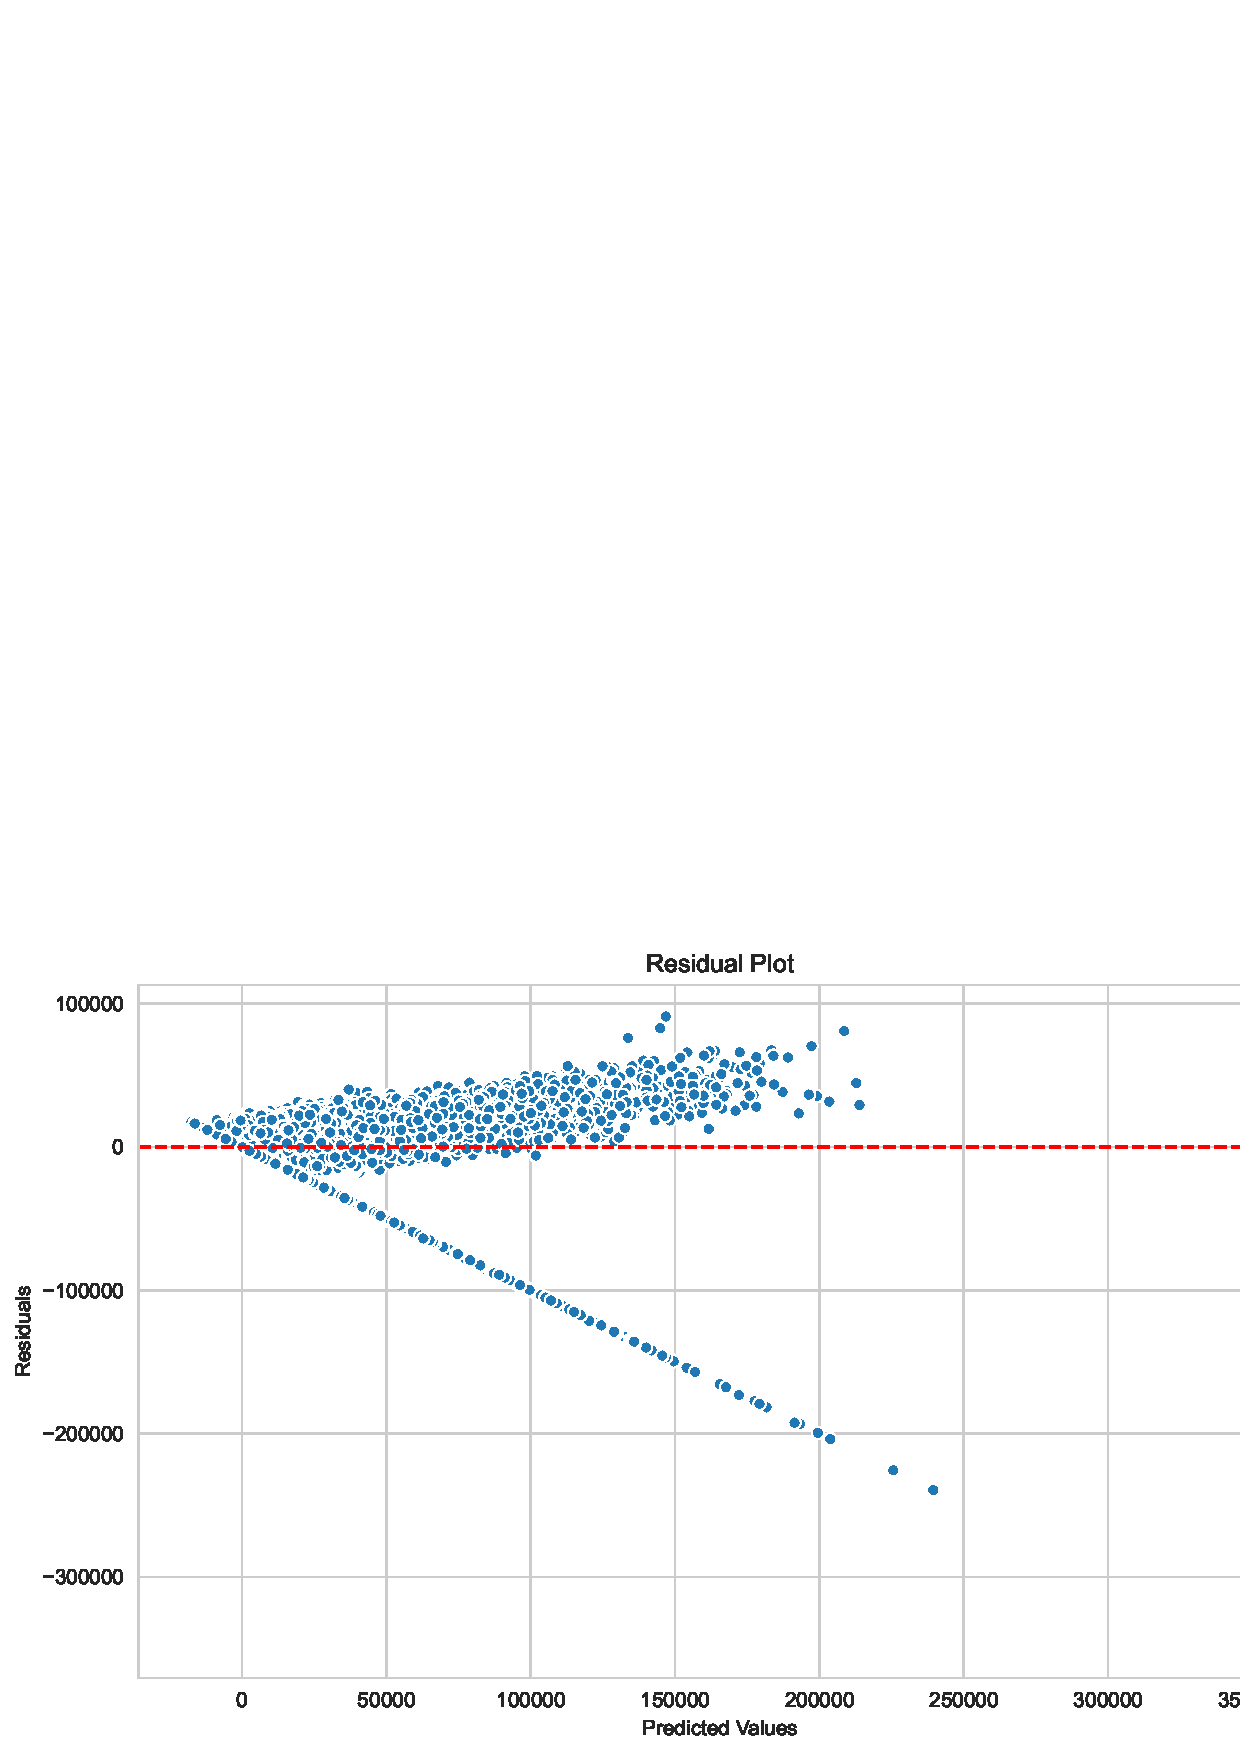
\includegraphics[width=0.7\textwidth]{plots/png/residual_plot.png}
    \caption{Residual Plot}
\end{figure}

\subsection*{5.3 Training vs Validation Error}
\begin{figure}[H]
    \centering
    \includegraphics[width=0.7\textwidth]{plots/png/learning_curve_Linear_Regression.png}
    \caption{Learning Curve - Linear Regression}
\end{figure}
\begin{figure}[H]
    \centering
    \includegraphics[width=0.7\textwidth]{plots/png/learning_curve_Ridge_Regression.png}
    \caption{Learning Curve - Ridge Regression}
\end{figure}

\subsection*{5.4 Coefficient Analysis}
\begin{figure}[H]
    \centering
    \includegraphics[width=0.8\textwidth]{plots/png/coefficients_comparison.png}
    \caption{Top Feature Coefficients Comparison}
\end{figure}

%==================================================
\section*{Performance Metrics to be Reported}
\begin{itemize}
    \item Mean Absolute Error (MAE)
    \item Mean Squared Error (MSE)
    \item Root Mean Squared Error (RMSE)
    \item $R^2$ Score
    \item Training Time
\end{itemize}

%==================================================
\section*{Hyperparameter Search Space}
\begin{itemize}
    \item Ridge: $\alpha \in \{0.01, 0.1, 1, 10, 100\}$
    \item Lasso: $\alpha \in \{0.001, 0.01, 0.1, 1, 10\}$
    \item Elastic Net:
    \begin{itemize}
        \item $\alpha \in \{0.01, 0.1, 1, 10\}$
        \item $l1\_ratio \in \{0.2, 0.5, 0.8\}$
    \end{itemize}
\end{itemize}

%==================================================
\section*{Hyperparameter Tuning Results}
\begin{table}[h!]
\centering
\renewcommand{\arraystretch}{1.3}
\caption{Hyperparameter Tuning Summary}
\begin{tabular}{|l|c|c|c|}
\hline
Model & Search Method & Best Parameters & Best CV $R^2$ \\ \hline
Ridge Regression & Grid Search & $\alpha=100$ & 0.5847 \\
Lasso Regression & Grid Search & $\alpha=10$ & 0.5840 \\
Elastic Net Regression & Grid Search & $\alpha=0.1, l1\_ratio=0.8$ & 0.5872 \\ \hline
\end{tabular}
\end{table}

%==================================================
\section*{Cross-Validation Performance (K = 5)}
\begin{table}[h!]
\centering
\renewcommand{\arraystretch}{1.3}
\caption{Cross-Validation Performance (Validation Set)}
\begin{tabular}{|l|c|c|c|c|}
\hline
Model & MAE & MSE & RMSE & $R^2$ \\ \hline
Linear Regression & 21588.53 & 1019214563 & 31925.14 & 0.5510 \\
Ridge Regression & 21582.04 & 1017453676 & 31897.55 & 0.5517 \\
Lasso Regression & 21564.42 & 1017939233 & 31905.16 & 0.5515 \\
Elastic Net Regression & 21642.32 & 1016502099 & 31882.63 & 0.5522 \\ \hline
\end{tabular}
\end{table}

%==================================================
\section*{Test Set Performance Comparison}
\begin{table}[h!]
\centering
\renewcommand{\arraystretch}{1.3}
\caption{Test Set Performance}
\begin{tabular}{|l|c|c|c|c|}
\hline
Model & MAE & MSE & RMSE & $R^2$ \\ \hline
Linear Regression & 21588.53 & 1.02e9 & 31925.14 & 0.5510 \\
Ridge Regression (Tuned) & 21582.04 & 1.01e9 & 31897.55 & 0.5517 \\
Lasso Regression (Tuned) & 21564.42 & 1.01e9 & 31905.16 & 0.5515 \\
Elastic Net Regression (Tuned) & 21642.32 & 1.01e9 & 31882.63 & 0.5522 \\ \hline
\end{tabular}
\end{table}

%==================================================
\section*{Effect of Regularization on Coefficients}
\begin{table}[h!]
\centering
\renewcommand{\arraystretch}{1.3}
\caption{Coefficient Comparison}
\begin{tabular}{|l|c|c|c|c|}
\hline
Feature & Linear & Ridge & Lasso & Elastic Net \\ \hline
Loan Amount Request & 35357.49 & 35248.81 & 35345.98 & 29622.79 \\
Income (USD) & 34525.04 & 1421.13 & 33816.66 & 176.99 \\
Property Age & -34464.71 & -1331.06 & -33758.38 & -122.04 \\
Credit Score & 11645.44 & 11625.56 & 11641.87 & 11529.83 \\ \hline
\end{tabular}
\end{table}

%==================================================
\section*{Overfitting and Underfitting Analysis}
The learning curves show that as training data increases, the training score decreases slightly while the validation score increases, converging to an $R^2$ of around 0.55 - 0.59. Deep gap between training score ($1.0$ at start) and validation indicates high variance initially, but they converge. However, the final score (~0.55) suggests moderate performance; the model might be slightly underfitting (high bias) given the complexity of real-world loan data, or the features provided are not fully sufficient to predict the exact loan amount. Regularization (especially Elastic Net) provided a marginal improvement, suggesting that overfitting was not the primary issue, but it successfully stabilized the coefficients (e.g., drastically reducing 'Income' coefficient which was inflated in Linear Regression).

%==================================================
\section*{Bias--Variance Analysis}
Linear Regression exhibits high variance in coefficient estimates (very large values due to multicollinearity between Income and possibly other features). Ridge and Elastic Net successfully reduced this variance by shrinking coefficients (Bias increased slightly, but Variance decreased significantly). Lasso performed feature selection but behaved similarly to Linear for some features. Elastic Net provided the best trade-off, achieving the lowest RMSE and highest $R^2$.

%==================================================
\section*{Conclusion}
In this experiment, Elastic Net Regression achieved the best performance with an $R^2$ of 0.5522 and RMSE of 31882.63. Plain Linear Regression suffered from multicollinearity, evidenced by massive coefficients for 'Income' and 'Property Age' which were effectively neutralized by Ridge and Elastic Net regularization. While the improvement in metrics was small, the improvement in model stability and interpretability was significant. The results highlight the importance of regularization in handling correlation among features in regression tasks.

%==================================================
\section*{References}
\begin{itemize}
    \item \href{https://scikit-learn.org/stable/modules/linear_model.html}{Scikit-learn: Linear Models}
    \item \href{https://scikit-learn.org/stable/modules/grid_search.html}{Scikit-learn: Hyperparameter Optimization}
    \item \href{https://www.kaggle.com/datasets/phileinsophos/predict-loan-amount-data}{Loan Amount Dataset}
\end{itemize}

\end{document}
